\section{Strategies for Addressing Identification Challenges}
\label{sec: what_can_we_do}

Although counterbalanced within‐subjects designs present some identification challenges, there are practical strategies available to researchers to address these problems. This section outlines five approaches—Fisher's Exact Test, heuristic checks, the use of a washout period, covariate adjustment, and using Sequential Randomization as described in Section \ref{sec: seq_exchangeability_alt_design}—that can help detect violations of the assumptions or satisfy them needed for consistent estimation of the causal effect.

\subsection{Fisher's Exact Test}

Fisher's Exact Test is a nonparametric method widely used to assess the independence between two categorical variables, making it particularly useful in small sample settings. In a \cwsd{}, if there is concern that assumption violations may be contaminating the analysis, one strategy is to discard data from $t_2$ and focus exclusively on $t_1$. By doing so, researchers can use Fisher's Exact Test at $t_1$ to determine whether the treatment assignment is independent of the observed outcomes.

However, this approach does not address the issue of limited overlap and lack of common support, which may arise with the sample sizes typically used in \cwsd{}. Therefore, while it is a viable option, the experimenter may still need to ensure covariate balance at $t_1$, and its applicability may be limited in certain contexts.

\subsection{Heuristics Checks}

A straightforward diagnostic is to compare the estimated treatment effect in the first period, \(\hat{\tau}_{t_1}\), to the estimated effect in the second period, \(\hat{\tau}_{t_2}\). A marked discrepancy between these estimates may indicate violations of the no‐carryover or no‐time‐drift assumptions (analogous to pre‐trend checks in a difference‐in‐differences setting).

When large differences emerge, they serve as a clear warning sign that carryover or other time‐based confounders may be at play.  However, consistency between \(\hat{\tau}_{t_1}\) and \(\hat{\tau}_{t_2}\) does not guarantee the validity of the requisite assumptions: random sampling variability could mask carryover effects, while strongly offsetting biases might also produce superficially similar estimates. Inconsistencies between the estimates also do not imply that the assumptions are violated as differences might arise due to sampling variability. As such, this check is neither necessary (i.e., estimates may differ for benign reasons) nor sufficient (i.e., matching estimates could still reflect compensating biases).

Despite these limitations, heuristic checks remain a useful first step in diagnosing possible threats to identification and can guide further analyses. However, given that \cwsd{} is often employed due to a small sample size, in practice, it can be difficult to determine that difference in estimates is driven by the violation of the assumptions, or sampling variation, or both.

\subsection{Washout Period}

A more targeted design‐based remedy is to incorporate a \textit{washout period} between treatments. This approach is particularly relevant when the treatment is expected to have direct physiological or psychological effects that persist over time, but decay with a sufficient gap between $t_1$ and $t_2$. By lengthening the gap between \(t_1\) and \(t_2\), the influence of the initial treatment on the second‐period outcome may subside, thereby reducing or eliminating any carryover effects.  

 Researchers should draw on subject‐matter knowledge (e.g., pharmacokinetics, psychological adaptation timelines) to determine the length of time needed for treatment effects to dissipate. Even with an adequate washout period, however, confounding due to the effect of treatment on the covariates remains a concern. If, for instance, the initial treatment induces behavioral or physiological changes that persist, mere passage of time may not fully remove indirect carryover pathways. Thus, the potential for lingering confounders should still be carefully addressed (e.g., by measuring and adjusting for relevant characteristics at \(t_2\)).


\subsection{Controlling for Changes in Covariates}

\begin{figure}[h]
    \centering
    \begin{subfigure}[b]{0.45\textwidth}
    \tikz{
        \node (space) at (0,1) {};
        \node (space) at (0,-2) {};
        \node (Zt1) at (2,0) {$Z_{i,t_1}$};
        \node (Xt1) at (0,-1) {$X_{i,t_1}$};
        \node (Yt1) at (2,-1) {$Y_{i,t_1}$};
        
        \node (Zt2) at (4,0) {$Z_{i,t_2}$};
        \node (Xt2) at (4,-1) {$X_{i,t_2}$};
        \node (Yt2) at (6,0) {$Y_{i,t_2}$};
    
        \path[->, thick] (Xt1) edge (Yt1);
        \path[->, thick] (Zt1) edge (Yt1);
        \path[->, thick] (Zt1) edge (Zt2);
        \path[->, thick] (Yt1) edge (Xt2);
        \path[->, thick] (Zt2) edge (Yt2);
        \path[->, thick] (Xt2) edge (Yt2);
        %\path[->, thick] (Zt1) edge[out=30, in=150] (Yt2);
        \path[->, thick] (Zt1) edge (Xt2);
        \path[->, thick] (Xt1) edge[out=-30, in=-150] (Xt2);
    }
    \subcaption{Counterbalanced Within-Subjects}
    \label{fig: cwsd_dag_no_dir}
    \end{subfigure} \vspace{1mm}
    \begin{subfigure}[b]{0.45\textwidth}
    \tikz{
        \node (space) at (0,1) {};
        \node (space) at (0,-2) {};
        \node (Zt1) at (2,0) {$Z_{i,t_1}$};
        \node (Xt1) at (0,-1) {$X_{i,t_1}$};
        \node (Yt1) at (2,-1) {$Y_{i,t_1}$};
        
        \node (Zt2) at (4,0) {$Z_{i,t_2}$};
        \node (Xt2) at (4,-1) {$X_{i,t_2}$};
        \node (Yt2) at (6,0) {$Y_{i,t_2}$};
    
        \path[->, thick] (Xt1) edge (Yt1);
        \path[->, thick] (Zt1) edge (Yt1);
        \path[->, thick] (Yt1) edge (Xt2);
        \path[->, thick] (Zt2) edge (Yt2);
        \path[->, thick] (Xt2) edge (Yt2);
        %\path[->, thick] (Zt1) edge[out=30, in=150] (Yt2);
        \path[->, thick] (Zt1) edge (Xt2);
        \path[->, thick] (Xt1) edge[out=-30, in=-150] (Xt2);
    }
    \subcaption{Sequential Randomization}
    \label{fig: sr_dag_no_dir}
    \end{subfigure}
    \caption{Assuming that all carryover effects are mediated by the covariates at the second time period, failing to control for $X_{i,t_2}$ will lead to biased estimates in a \cwsd{}. However, this is not true for Sequential Randomization. Note that $X_{i,t_1}, X_{i,t_2}$ includes both observed and unobserved covariates for concision.}
    \label{fig:CWSD_DAG_Without_Direct}
\end{figure}

If the carryover effect is entirely mediated by observable covariates at the second time period, \(X_{i,t_2}\) (i.e., if all carryover effects operate indirectly through these covariates), then adjusting for \(X_{i,t_2}\) fully accounts for any such indirect influence. Formally, controlling for the covariates at $t_2$ satisfies Assumption \ref{assumption: sequential_exchangeability: ignorability_t2}.

To illustrate with the Ozempic experiment, suppose that any direct carryover effects of the treatment on blood sugar levels at \(t_1\) become negligible following an appropriate washout period; then the assumption of no direct carryover effects becomes more credible. However, if participants assigned to Ozempic continue to maintain elevated physical activity relative to those in the control group, a \cwsd{} will violate Assumption \ref{assumption: sequential_exchangeability: ignorability_t2}.

To account for this in a \cwsd{}, we can adapt methods from observational causal inference by adjusting for $X_{i,t_2}$ using regression models or propensity score weighting. These approaches block indirect pathways through which prior treatment might influence the outcome. In contrast, a simple time dummy only captures average period effects and fails to account for treatment–covariate interactions. Nevertheless, while such adjustments are theoretically viable in a \cwsd{}, they may be difficult to implement in practice, and model misspecification can introduce bias. Therefore, even when direct carryover effects seem unlikely or negligible, we recommend using sequential randomization as described in Section \ref{section: alternative_designs}.

To demonstrate this, we simulated a \cwsd{} where participants were randomized to sequences, and varied the effect of the effect of $Z_{t_1}$ on $X_{t_2}$ from –10 to 10. We estimated the treatment effect using four methods: a correctly specified model, a propensity score method, a fixed time effect model, and an unadjusted model. 

As shown in Figure \ref{fig:simulation_cwsd}, only the correctly specified and propensity score models consistently recovered the true treatment effect. The fixed effect and unadjusted models produced biased estimates, with bias increasing alongside the treatment’s effect on the covariates. We repeated the simulation using sequential randomization, which yielded unbiased estimates regardless of model (mis)specification.


\begin{figure}[h]
    \centering
    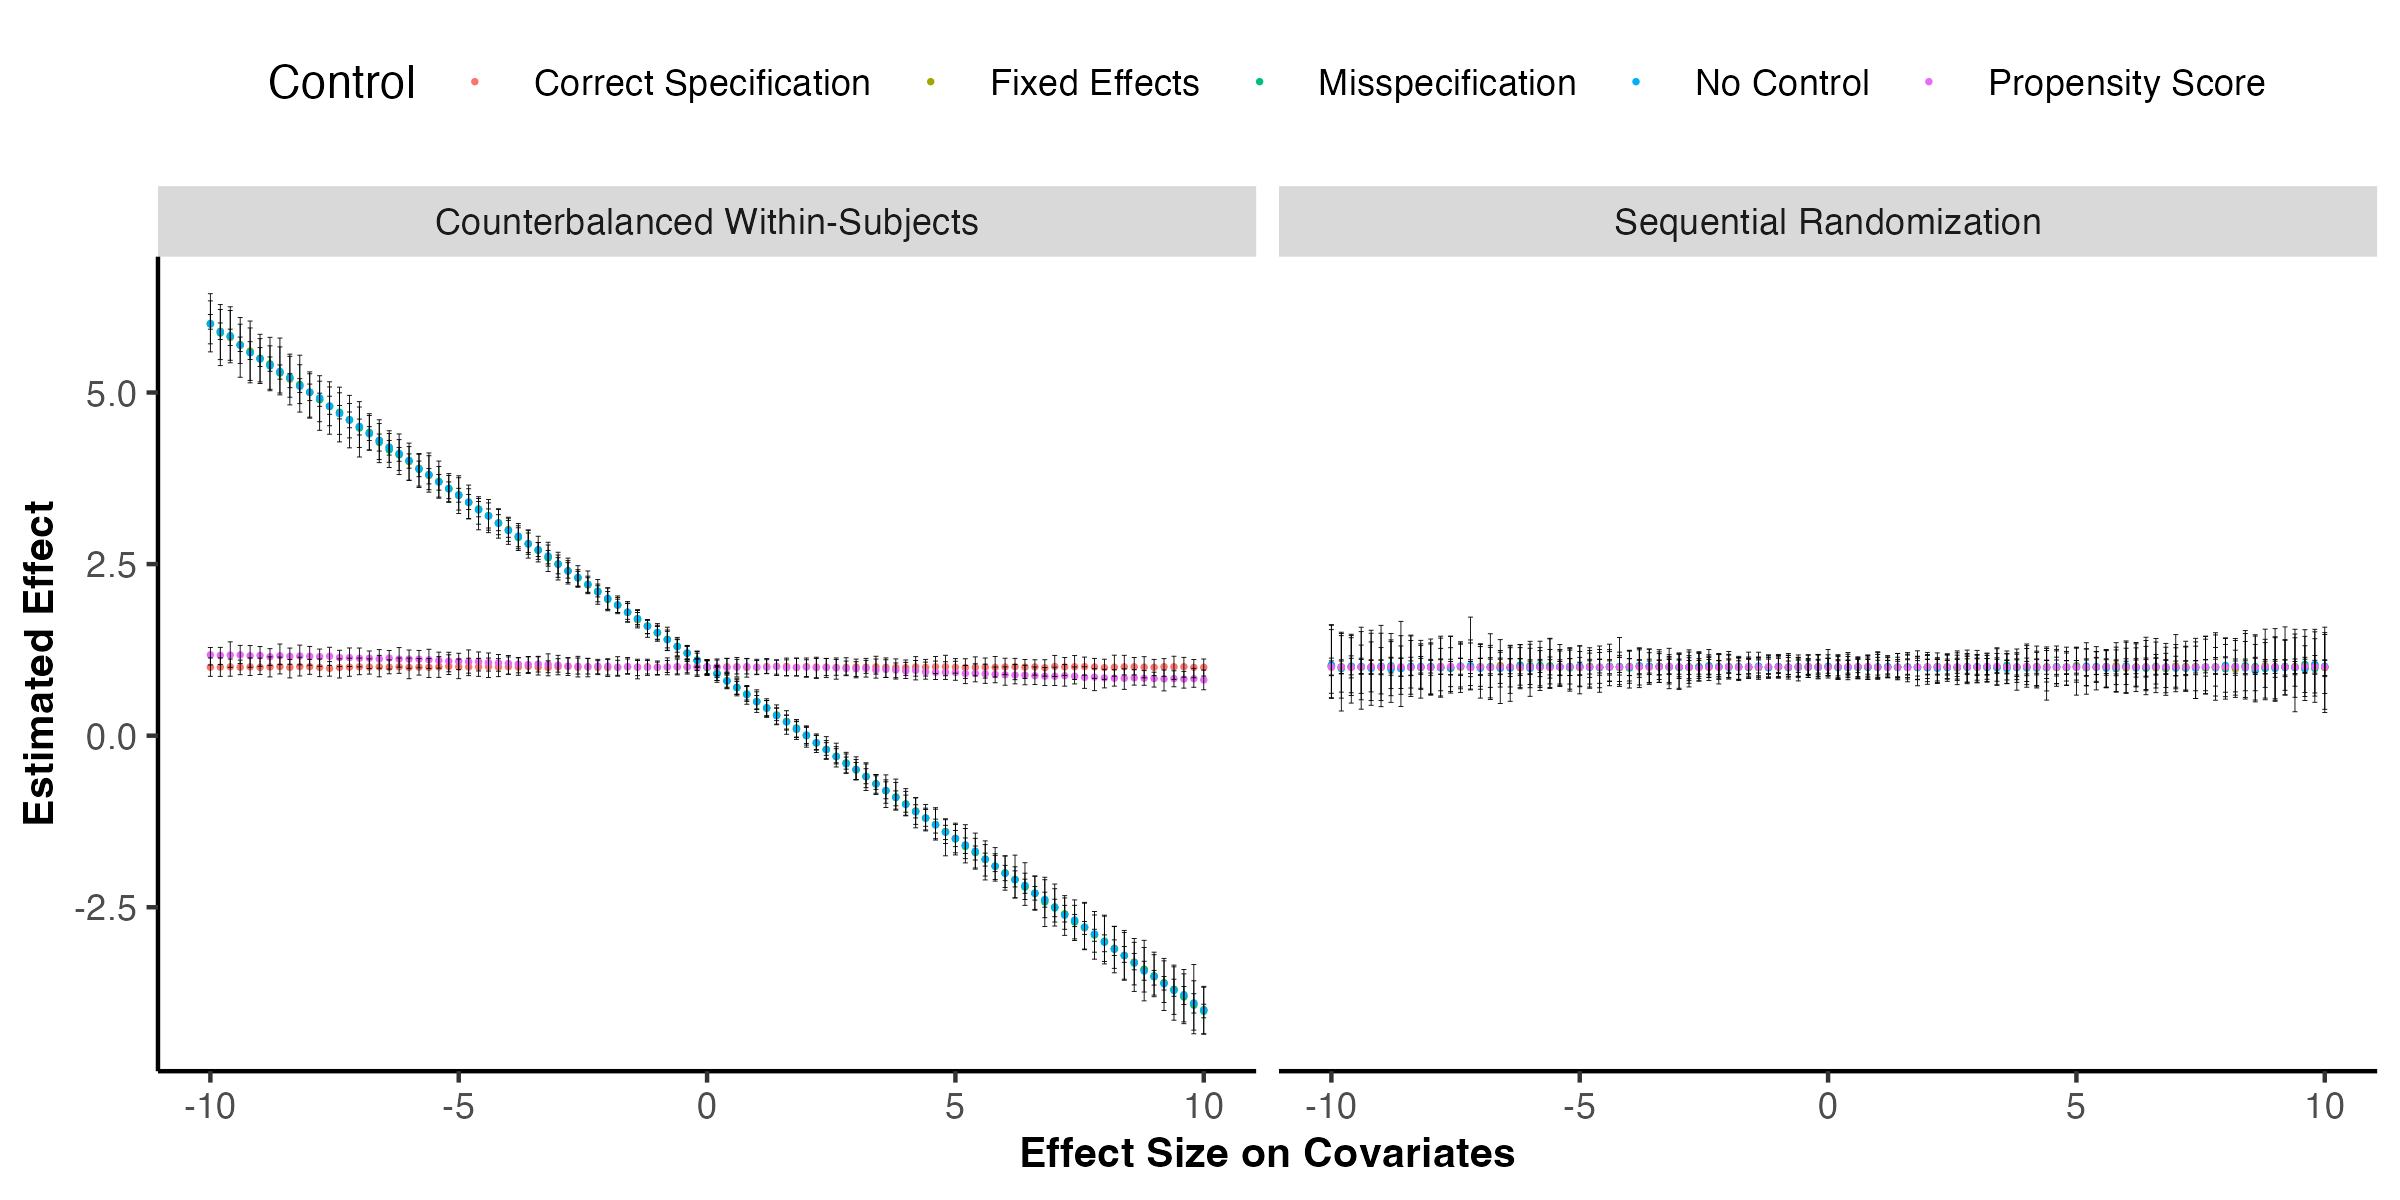
\includegraphics[width=0.95\linewidth]{Figures/Design_Comparison.png}
    \caption{Simulated estimates of the treatment effect \(\tau = 1\) obtained using different estimation methods. In the \cwsd{} simulation, both the Correct Specification and Propensity Score approaches successfully recovered the unbiased treatment effect, while the Fixed Effects and No Control methods introduced bias. The degree of bias in the Fixed Effects and No Control approaches increased as the effect size on the covariates grew. Nonetheless, a sequential randomization design consistently recovered the average treatment effect (ATE) regardless of the specification.}
    \label{fig:simulation_cwsd}
\end{figure}

Although adjusting for covariates at $t_2$ can help block indirect carryover pathways, care must be taken not to condition on previous treatment outcomes such as \( Y_{i,t_1} \). In particular, consider the path \[ Z_{i,t_2} \leftarrow Z_{i,t_1} \rightarrow Y_{i,t_1} \leftarrow X_{i,t_1} \rightarrow X_{i,t_2} \rightarrow Y_{i,t_2} \] $Y_{i, t_1}$ is a collider and conditioning on it opens a non-causal backdoor path from \( Z_{i,t_1} \) to \( Y_{i,t_2} \). This violates the backdoor criterion and introduces what is known as collider bias or \textit{M}-bias \citep{21_M_Bias, 22_good_and_bad_crtl}. As a result, estimates of the causal effect may become biased. Thus, in a \cwsd{}, treatment outcomes at $t_1$ should not be conditioned on when estimating causal effects of \( Z_{i,t_2} \) on $Y_{i,t_2}$.